Determine todos os valores de $n$ tais que é possível dividir um triângulo em $n$ triângulos de
modo que não haja três vértices alinhados e em cada vértice incida o mesmo número de
segmentos.

Mostramos a seguir tal divisão para $n = 7$. Observe que em cada um dos seis vértices incidem
quatro segmentos.

\begin{center}
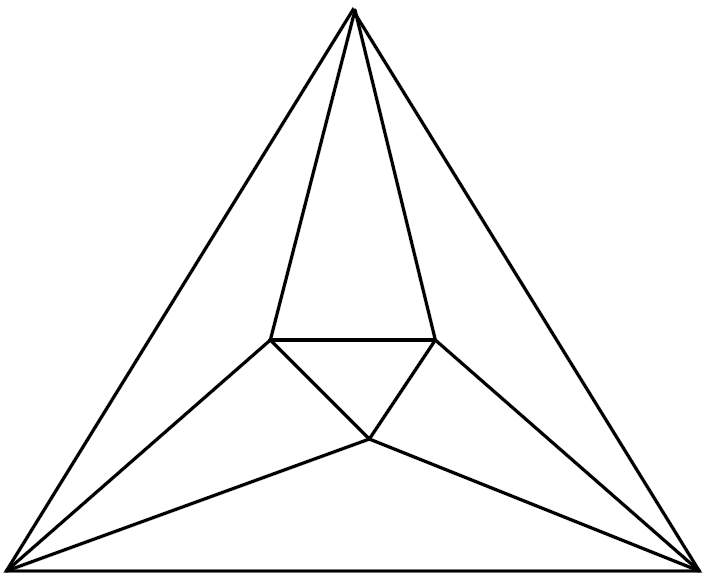
\includegraphics[width = 4cm]{figura.png}
\end{center}